%%%%%%%%%%%%%%%%%%%%%%%%%%%%%%%%%%%
%%                               %%
%% Špeciálne a netextové objekty %%
%%                               %%
%%%%%%%%%%%%%%%%%%%%%%%%%%%%%%%%%%%
\chapter{Špeciálne a netextové objekty}
\section{Matematické rovnice}
Systém na sadzbu textu \TeX\ pôvodne vyvinul Donald Knuth.
Jeho motivácia bola poskytnúť producentom vedeckej tlače
počítačový nástroj,
ktorý bude správne sádzať matematické rovnice.
\LaTeX, ako jeho nadstavba, má sadzbu rovníc takpovediac
v~genetickej výbave.
Autori textov z prírodovedeckej a technickej komunity siahajú po tomto nástroji
práve z~dôvodu bezkonkurenčnej práce s~rovnicami pri tvorbe
vedeckého alebo akademického obsahu.

Matematické rovnice používame v tlačenom texte dvomi spôsobmi:
1. píšeme ich v~rámci textového odseku;
2. rovnicu vytlačíme zvlášť medzi dva textové odseky
a~vtedy ju spravidla aj číslujeme, aby sme sa na ňu mohli
ďalej odvolávať.

\subsection{Rovnica v textovom riadku}
Riešenie kvadratickej rovnice s koeficientami $a,b,c$
a~s~neznámou $x$ vypočítame pomocou známeho vzťahu
$x=\frac{-b\pm\sqrt{b^2-4ac}}{2a}$.
Je to príklad rovnice zapísanej v~rámci textového odseku.
Ak tú istú rovnicu napíšeme do samostatného odseku,
vyzerá trochu inak:
$$
  x=\frac{-b\pm\sqrt{b^2-4ac}}{2a}
$$

Očividný rozdiel je vo veľkosti zlomku a~znaku odmocniny,
môžeme si všimnúť aj malé rozdiely v~medzerách,
vo vertikálnom zarovnávaní, atď.

Vložené rovnice v~rámci textového riadku zapisujeme pomocou
znaku \$.
Matematický zápis ohraničíme znakmi dolára sprava aj zľava.
Napríklad zápis \verb|$y = ax^2 + bx + c$| vytvorí rovnicu $y = ax^2 + bx + c$. Rovnakú funkciu ako znak dolára má dvojica znakov \verb|\(...\)|.

Označenia fyzikálnych veličín píšeme tiež ako vloženú rovnicu:
veľkosť sily $F$, hmotnosť $m$, čas $t$ a~podobne.
Všetky veličiny sme zapísali takto: \verb|$F$|,
\verb|$m$|, \verb|$t$|.

\subsection{Zobrazená rovnica}
Matematický text ohraničený dvomi znakmi dolára zľava
a~dvomi dolármi sprava interpretuje kompilátor \LaTeX-u
ako zobrazenú rovnicu, ktorú vysádza do zvláštneho odseku
zarovnaného na stred, napríklad
$$
  y = ax^2 + bx + c
$$
sme získali kódom \verb|$$y = ax^2 + bx + c$$|.
Namiesto dolárov môžeme použiť dvojicu príkazov
\verb|\[...\]| s rovnakým výsledkom.

Rovnicu s referenčným číslom vytvoríme tak, že zápis matematickej
rovnice vložíme do prostredia \verb|equation|:
\begin{verbatim}
  \begin{equation}
    y = ax^2 + bx + c
  \end{equation}
\end{verbatim}
vytvorí rovnicu s číslom uzavretým v zátvorkách:
\begin{equation}
  y = ax^2 + bx + c
\end{equation}

Program \LaTeX\ čísluje rovnice automaticky od čísla 1.

\subsection{Zásady matematickej sadzby}
Pravidlá sadzby matematických, fyzikálnych veličín a~ich vzťahov
sumarizuje medzinárodná norma u~nás známa pod označením
STN ISO 80 000: 2022 Veličiny a~jednotky \cite{iso800001, iso800002}.
Označenie fyzikálnych a~matematických veličín píšeme vždy
šikmým rezom písma.
Čísla, názvy funkcií a~jednotky fyzikálnych veličín zapisujeme
normálnym rezom.
Správny zápis elektrického napätia s veľkosťou 5,07 voltu
vyzerá takto:
\begin{equation}\label{Eq:quantity}
  U = 5{,}07\,\mathrm{V}
\end{equation}
kde $U$ je elektrické napätie.
Môžeme si všimnúť, že okolo znaku rovnosti sú medzery,
desatinná čiarka sa píše bez medzier a~medzi číslom a~jednotkou
je úzka medzera -- v~\LaTeX-u príkaz \verb|\,|.

Rovnicu (\ref{Eq:quantity}) sme zapísali v zdrojovom kóde nasledujúcim spôsobom:
\begin{verbatim}
\begin{equation}
  U = 5{,}07\,\mathrm{V}
\end{equation}
\end{verbatim}
\TeX\ v~matematickom móde automaticky sádže veličiny kurzívou.
Ak chceme, aby bola jednotka V vzpriamená, použijeme
v~matematickom móde príkaz \verb|\mathrm{}|. Medzery okolo znaku rovnosti sú taktiež automatické.
Zaujímavá je desatinná čiarka, ktorú musíme uzavrieť do
zložených zátvoriek, aby sme potlačili automatickú sadzbu
medzery za čiarkou.
V~anglicky hovoriacich krajinách sa ako desatinný oddeľovač
používa bodka.
Čiarka má väčšinou význam oddeľovača prvkov zoznamov
a~v~matematickom režime vkladá \TeX\, za čiarku úzku medzeru.
Najčastejšie chyby pri zápise fyzikálnych veličín sme zhrnuli
v~tabuľke 1.

\begin{table}[h]
\centering
\caption{Prehľad najčastejších chýb pri nesprávnom zápise
skalárnej fyzikálnej veličiny.
Správny zápis predstavuje rovnica (\ref{Eq:quantity}).}
\vspace{12pt}
\begin{tabular}{@{}ll@{}}
  \toprule
  \textbf{nesprávny zápis} & \textbf{opis chyby}\\
  \midrule
  $U = 5{,}07\,V$ & jednotka je kurzívou\\
  $U = 5{,}07\mathrm V$ & medzi číslom a jednotkou chýba medzera\\
  $\mathrm U = 5{,}07\,\mathrm V$ & označenie veličiny nie je kurzívou \\
  $U$=$5{,}07\,\mathrm V$ & okolo znaku rovnosti chýbajú medzery\\
  $U = 5,07\,\mathrm{V}$ & za desatinnou čiarkou je medzera\\
  $U = \mathit{5{,}07}\,\mathrm{V}$ & číslo je kurzívou\\
  U=$\mathit{5,07}V$ & kumulácia predchádzajúcich chýb\\
  \bottomrule
\end{tabular}
\end{table}

\subsubsection{Dôležité pravidlá písania rovníc}
\begin{itemize}

    \item Značky veličín píšeme šikmým rezom písma (kurzívou):
    $x$, $y$, $a$, $F$, $P$, $W$.

    \item Fyzikálne jednotky píšeme vzpriameným písmom:
    $a = 10\,\mathrm{cm}$.

    \item Čísla píšeme vzpriameným písmom:
    $1$; $2$; $3$; $1\,024$; $3{,}14$ a podobne.

    \item Skratky matematických funkcií píšeme vzpriameným
    písmom: $\sin(\alpha + \beta)$, $\cos\omega t$,
    $\log_a x = \frac{\ln x}{\ln a}$, $\mathrm{e^{i\uppi}}=-1$.

    \item Označenia nemenných konštánt sú tiež vzpriamené
    písmená: $\uppi$, $\mathrm i$, $\mathrm e$ --
    tri základné matematické konštanty --
    Ludolfovo číslo, komplexná jednotka a~Eulerovo číslo.
    Niektoré konštanty sa zo zvyku môžu písať kurzívou,
    napríklad $\pi$ alebo dielektrická konštanta $\varepsilon_0$.
    Komplexná jednotka je však vždy vzpriamená:
    $\mathrm i^2 = -1$.

    \item Vzpriameným písmom píšeme v matematických vzťahoch
    aj všetky zátvorky.

    \item Sumačné indexy píšeme kurzívou:
    $p_N(x) = \sum_{i=1}^N a_ix^i$.
    Symbol $i$ v tomto príklade predstavuje sumačný index,
    nie komplexnú jednotku.

    \item Vektory uvádzame buď polotučným šikmým rezom
    ($\vectorsym a$, $\vectorsym b$, $\vectorsym F$)
    alebo šikmým netučným rezom so šípkou nad symbolom:
    $\vec a$, $\vec b$, $\vec F$.
    Treba si vybrať jeden spôsob a~ten používať v~celej práci.

    Označenia matíc a tenzorov zapisujeme polotučným šikmým rezom:
    $$\matrixsym M = \left( \begin{array}{cc}
                            m_{11} & m_{12}\\
                            m_{21} & m_{22}
                        \end{array}\right)
    $$
    Prvky matice $m_{ij}$ sú skalárne veličiny, preto sú to
    netučné šikmé písmená.

    \item Ak treba z nejakého dôvodu odlíšiť tenzor
    od bežnej matice, môžeme tenzory označiť dvomi čiarkami:
    $\overline{\overline T}$.

    \item Značku úplného diferenciálu píšeme vzpriameným rezom:
    $\mathrm dy$ je úplný diferenciál veličiny $y$.

    \item Derivácia dráhy podľa času:
    $v = \frac{\mathrm ds}{\mathrm dt}$.
    Veličiny $v$, $s$ a~$t$ sú stále písané kurzívou

    \item Určitý integrál vyzerá takto:
    $$
    \int_a^b f(x)\,\mathrm dx
    $$
    V~integráli spravidla vkladáme pred diferenciál
    úzku medzeru \verb|\,|.
\end{itemize}

\subsection*{\normalsize Príklad}
Z Coulombovho zákona vyplýva,
že pre vektor elektrostatickej sily $\mathbfit F_\mathrm e$
medzi dvomi bodovými nábojmi platí nasledujúci vzťah
\begin{equation}\label{Eq:CoulombVec}
  \mathbfit F_\mathrm e = \frac1{4\pi\varepsilon_0}
  \frac{q_1q_2}{r^2}\frac{\mathbfit r}r
\end{equation}
kde $q_1$, $q_2$ sú veľkosti bodových nábojov,
$\mathbf r$ je polohový vektor náboja $q_2$
vzhľadom na náboj $q_1$
a~$\varepsilon_0$ je elektrická konštanta.

Aby sme zhrnuli predchádzajúce pravidlá, detailnejšie opíšeme spôsob zápisu jednotlivých prvkov
v~rovnici (\ref{Eq:CoulombVec}).
Skalárne veličiny veľkosť náboja a~vzájomná vzdialenosť sú
napísané kurzívou,
vektorové veličiny sila a~polohový vektor sú polotučným rezom.
Všetky čísla (indexy a~násobok 4 v~menovateli)
píšeme normálnym rezom.
Konštanty $\pi$ a $\varepsilon_0$ sú podľa zvyklosti vysádzané
šikmým rezom.
Norma v~súčasnosti odporúča vzpriamené písmo:
$\uppi$, $\upvarepsilon_0$, čo možno dosiahnuť použitím balíka
\verb|upgreek|.
Index $\mathrm e$ pri symbole vektora sily,
ktorý označuje fakt, že ide o~elektrickú silu,
píšeme normálnym neskloneným rezom písma.

V~texte, ktorý nasleduje bezprostredne za rovnicou vysvetlíme
a~stručne opíšeme jednotlivé symboly.
Tento odsek formálne patrí k~rovnici,
preto nemá odsadený prvý riadok.
Ak to chceme dosiahnuť,
nevynecháme za rovnicou v~zdrojovom kóde
prázdny riadok.

Zdrojový kód rovnice \eqref{Eq:CoulombVec}:
\begin{verbatim}
\begin{equation}\label{Eq:CoulombVec}
  \mathbfit F_\mathrm e = \frac1{4\pi\varepsilon_0}
  \frac{q_1q_2}{r^2}\frac{\mathbfit r}r
\end{equation}
\end{verbatim}
Všimnite si, že niekedy argument funkcie nemusí byť
uzavretý zloženými zátvorkami (\verb|\mathrm e| je vo výsledku rovnaký ako \verb|\mathrm{e}|).
Tento fenomén je dôsledok priebehu kompilácie na úrovni tzv. procesorov \TeX-u.
Parameter bez zátvorky funguje správne vtedy,
ak je parameter práve jeden \emph{token}.%
\footnote{Čo je token? Je to akási najmenšia časť spracovaného
kódu, ktorý vstupuje do tzv. \emph{token procesora}
počas kompilácie.
Tokeny sú písmená, čísla, ale aj jednoduchý príkaz,
napr. \texttt{\textbackslash mathrm} je jeden token.
Problematika je síce komplexná, ale na pochopenie
toho, čo sa v~\TeX-u deje, dôležitá.
Existuje veľmi pekná kniha od Petra Olšáka \TeX book naruby z roku 2001 \cite{Olsak2001Texbook}.
Keďže sa už nedá zohnať, autor sa rozhodol, že ju sprístupní pre širokú verejnosť v digitálnej forme na stránke
\href{https://petr.olsak.net/tbn.html}{\texttt{petr.olsak.net/tbn.html}}.
}

%%%%%%%%%%%%%%%%%%%%%%%%%%%%%%%%%%%
%%                               %%
%% Obrázky, ilustrácie a tabuľky %%
%%                               %%
%%%%%%%%%%%%%%%%%%%%%%%%%%%%%%%%%%%
\section{Obrázky}
V akademickej oblasti prírodných a~technických vied sa v~záverečných prácach
objavujú v~pomerne veľkom počte aj netextové grafické objekty. Patria sem grafy, schémy, diagramy, fotografie,
prípadne iné dvojrozmerné vizualizácie obsahu.
Nehovoríme o~ozdobných grafických prvkoch,
tie do práce tohto typu nepatria.
Obsahové grafické prvky budeme spoločne nazývať slovom obrázok.
Obrázok môže byť súčasť textového odseku,
ale tejto možnosti sa vyhýbame,
ak to nie je úplne nevyhnutné.
Uprednostňujeme tzv. plávajúcu formu obrázkov,
teda objektov, ktoré sa nemusia nachádzať bezprostredne
na mieste v texte, kde sú spomenuté.
V zdrojovom kóde umiestňujeme príkazy na sadzbu obrázku za odsek,
v~ktorom sa o~ňom hovorí po prvýkrát.
Pod každým obrázkom je textové označenie,
začínajúce skratkou slova obrázok (Obr.) a~nasleduje
poradové číslo obrázku v práci.

Na obrázku \ref{fig:measurement} je znázornený proces správneho merania výšky dieťaťa.
Grafický objekt je súčasťou plávajúceho prostredia \verb|figure|.
Samotnú grafiku pripravíme v externom editore,
exportujeme ju do niektorého z bežných formátov (JPG, PNG, PDF)
a~jej vloženie do finálneho PDF súboru
záverečnej práce zariadi makro
\verb|\includegraphics| z~balíka \verb|graphix|.
Automatické číslovanie má na starosti príkaz \verb|\caption|,
ktorého argument je text pod obrázkom.
\begin{verbatim}
\begin{figure}[!ht]
    \centering
    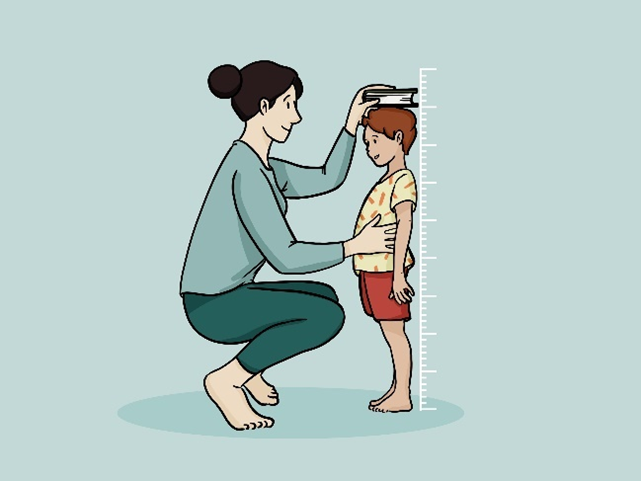
\includegraphics[scale=1.00]{img/Measurement.png}
    \caption{Pravidelné meranie výšky dieťaťa}
    \label{fig:measurement}
\end{figure}
\end{verbatim}

\begin{figure}[!ht]
    \centering
    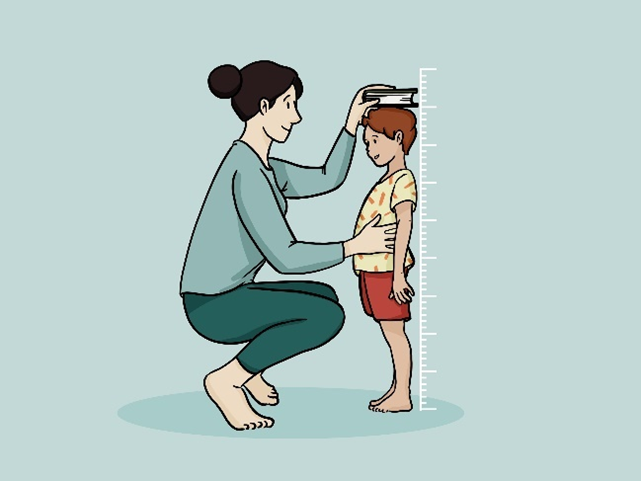
\includegraphics[scale=1.00]{img/Measurement.png}
    \caption{Pravidelné meranie výšky dieťaťa}
    \label{fig:measurement}
\end{figure}

\subsection{Umiestnenie obrázkov}\label{sec:figPlacement}
Na obrázok sa v~texte odkazujeme prostredníctvom čísla.
Môžeme písať o~tom, že na obrázku 1 vidíme to a~to
alebo použijeme skratku -- obr. 1.
Slovo obrázok aj skratku píšeme v~odkaze v~texte
malým začiatočným písmenom, ak sa nachádza vo vnútri vety.
Na každý obrázok v~práci by mal existovať odkaz v~texte.

Umiestnenie obrázku v rámci dokumentu riadi pomerne
komplikovaný algoritmus, čo nie vždy vedie k uspokojivým výsledkom.
Polohu plávajúceho objektu môžeme čiastočne ovplyvniť
nepovinným parametrom prostredia \verb|figure|.
V príklade, ktorý sme uviedli si môžeme všimnúť prítomnosť parametra \verb|h!| v hranatých zátvorkách
na konci prvého riadka.
Predstavuje požiadavku, že preferujeme,  aby sa obrázok nachádzal vo výslednom dokumente presne na tomto mieste. \LaTeX\ niekedy umiestni obrázok na začiatok nasledujúcej strany, prípadne aj inam.
Ak sa mu obrázok nepodarí umiestniť, zaradí ho až na
samý koniec kapitoly aj spolu so všetkými nasledujúcimi obrázkami.
To nebýva žiaduce a žiaľ, nemáme príliš veľa možností, ako takýto výsledok ovplyvniť.
Pomôže zmena rozmerov obrázku, prípadne jeho premiestnenie inam v zdrojovom kóde.
Odporúča sa, aby sa prostredie \verb|\begin{figure}...\end{figure}| nachádzalo mimo textového odseku, t. j. treba ho od okolitého textu oddeliť minimálne jedným prázdnym riadkom zhora aj zdola.

Na ovládanie umiestnenia plávajúceho objektu môžeme použiť tieto
parametre \verb|h|~(here) -- umiestnenie v mieste výskytu,
\verb|t|~(top) -- umiestnenie na stránke hore, \verb|b|~(bottom) --
umiestnenie na stránke dole, \verb|p|~(page) -- umiestnenie
na samostatnej stránke na konci kapitoly. Prvé tri
parametre môžu byť doplnené znakom výkričníka (\verb|!|),
ktorý požiadavku zosilňuje.
Jednotlivé parametre možno aj kombinovať.
Napríklad inštrukcia \verb|[!ht]| znamená, že chceme mať
obrázok na tom mieste, kde sa nachádza v zdrojovom kóde
a~ak to za žiadnu cenu nie je možné,
trebárs z~dôvodu nedostatku miesta pred koncom strany,
môže sa obrázok nachádzať aj v~hornej časti stránky.
Ani to však nemusí stačiť a~obrázok napokon nájdeme
na konci dokumentu.
V~takom prípade treba skúsiť niektoré
z~riešení spomenutých v~predchádzajúcom odseku.

\subsection{Označenie obrázku a text pod obrázkom}
Text pod obrázkom pozostáva z~označenia obrázku a z~vysvetľujúceho obsahu.
Mal by sa nachádzať spolu s~obrázkom na tej istej strane.

Text je dostatočne opisný,
aby bol jasný obsah obrázku aj pri rýchlom prechádzaní
práce bez nutnosti detailného čítania hlavného textu.
Ak opis pod obrázkom pozostáva iba z~jednej vety,
prípadne ide o~heslo bez vetnej štruktúry,
nepíšeme zaň bodku.
V~prípade viacerých viet už bodku alebo príslušné interpunkčné
znamienka použijeme na konci každej vety,
aj poslednej.
V príklade na obrázku \ref{fig:measurement} je text bez bodky
a~to je správne.

\subsection{Číslovanie a odkazy}
Obrázky číslujeme podľa výskytu v práci od čísla 1.
Používame jednoúrovňové číslovanie,
teda obrázok 1, obrázok 2, atď.
V~\LaTeX-u je automatické číslovanie obrázkov zabezpečené v definícii makra \verb|\caption|.

Odvolávanie sa na číslo obrázku rieši dvojica príkazov \verb|\label| a~\verb|\ref|.
Prvý príkaz zistí prítomnosť najbližšieho číselného
registra a priradí k nemu menovku, ktorú zadáme do argumentu.
Napríklad obrázok \ref{fig:measurement} má menovku \verb|fig:measurement|. Menovku volí autor textu, môže byť ľubovoľná, musí však začínať písmenom a nesmie obsahovať špeciálne znaky, ktoré majú v \TeX-u kategóriu vykonateľných príkazov (napr. \verb|\|, \verb|%|, \verb|#|, \verb|$|, zátvorky a podobne). Tiež treba venovať pozornosť tomu, aby sa rovnaká menovka nevyskytla v~texte v príkaze \verb|\label| viackrát, pretože by došlo k jej preťaženiu a znefunkčneniu odkazov.

Z praktických dôvodov sa ustálila prax začínať menovku skratkou typu číslovanej položky: \verb|fig| pre obrázok, \verb|eq| pri rovniciach, \verb|tab| ako menovka tabuľky, \verb|sec| v~prípade nadpisu, atď.

\section{Grafy}
Grafmi budeme nazývať zobrazenie vedeckých dát
najčastejšie vo forme dvojrozmerného grafu
závislosti dvoch alebo viacerých veličín.
Príklad takéhoto objektu je na obrázku \ref{fig:Graph1}.
Grafická reprezentácia vedeckých dát musí byť
v~prvom rade čitateľná, zreteľná a~jednoznačná.
Tomu treba prispôsobiť všetky zásady pri tvorbe grafov.

\begin{figure}[h!]
  \centering
  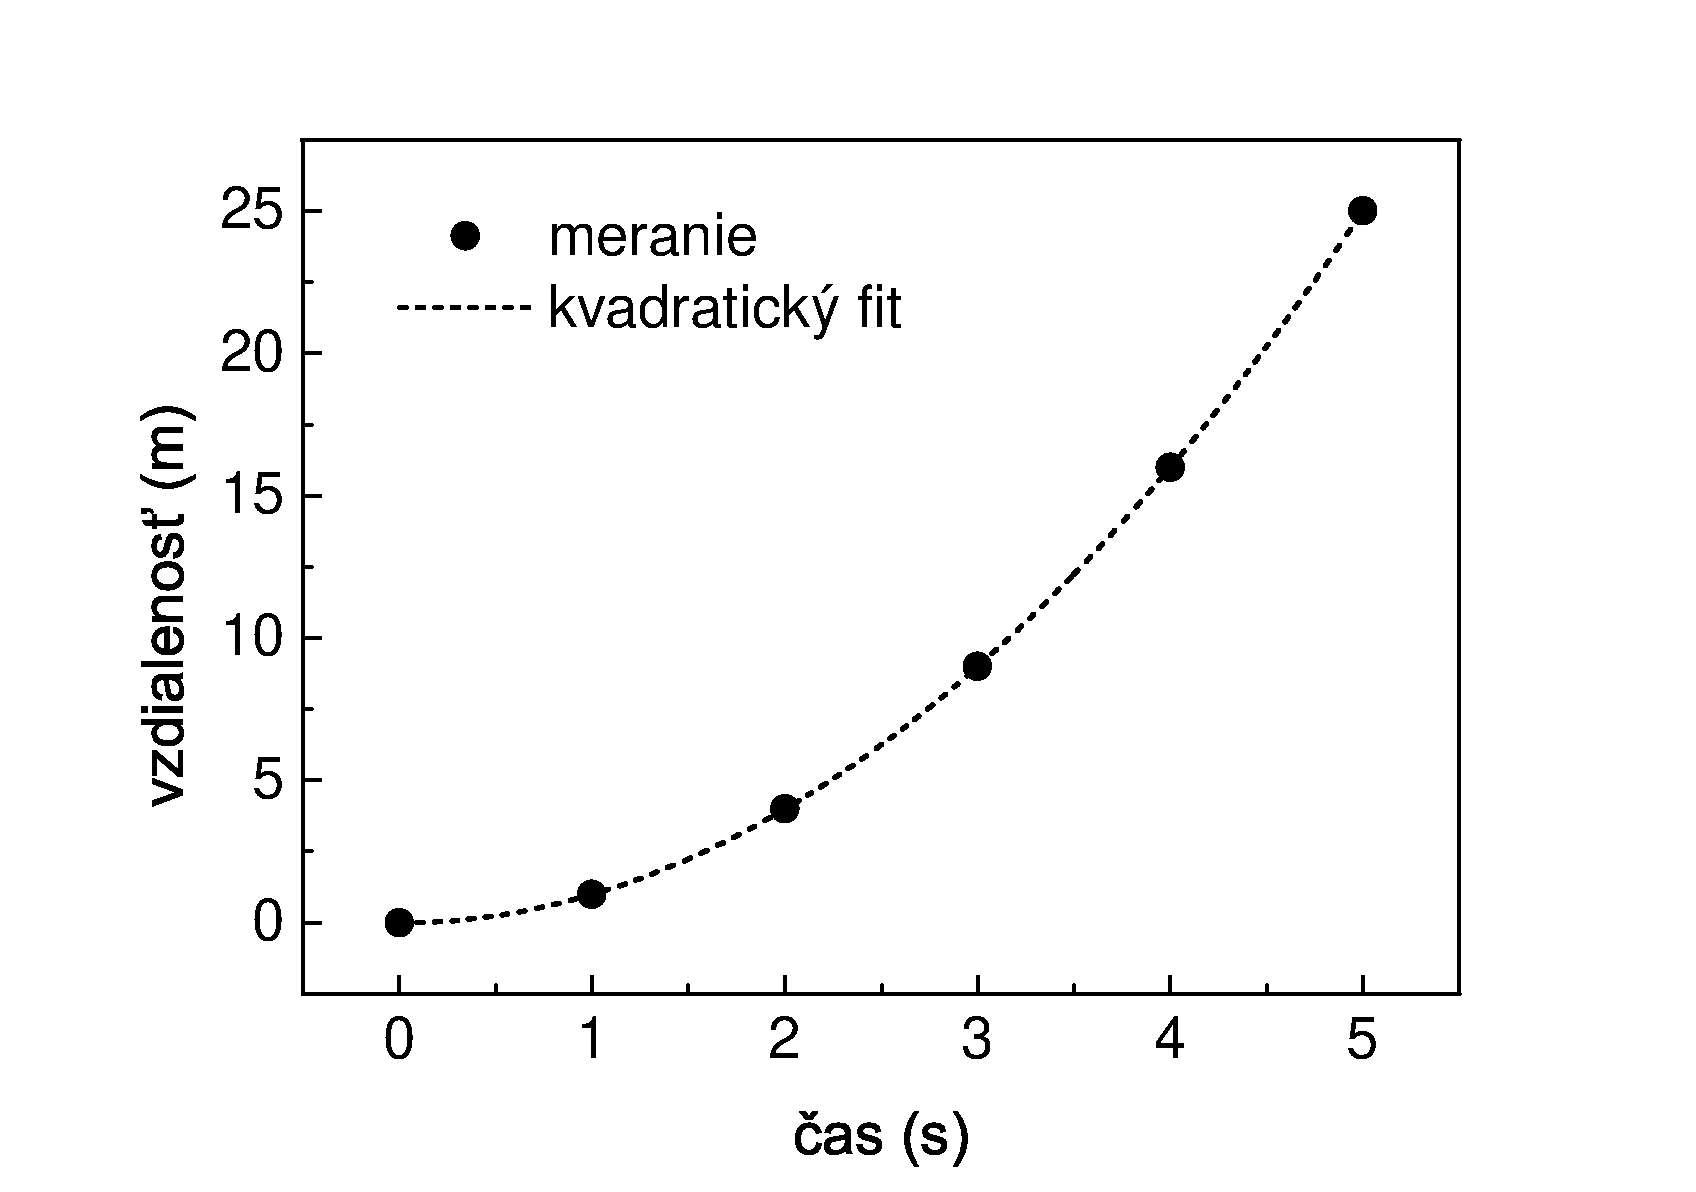
\includegraphics[scale=0.358]{img/Graph1}
  \caption{Ukážka grafu vytvoreného v externom programe a vloženého ako PDF súbor.
  Použité písmo je Arial s veľkosťou približne 10\,pt. Plné krúžky sú body merania a~prerušovaná čiara je kvadratický fit závislosti $s = at^2/2$, pričom $a = (2{,}00 \pm0{,}01)\,\mathrm{m\,s^{-2}}$.}
  \label{fig:Graph1}
\end{figure}

\subsection{Formát súboru}
Vektorové formáty SVG alebo PDF sú ideálna voľba pri exporte
z~grafických programov, napr. z~Excelu alebo Originu.
Ak takúto možnosť nemáme, treba grafy z externého softvéru
exportovať do bitmapového formátu, najlepšie PNG.
Stratový formát JPEG nie je na čiarovú grafiku vhodný.
Rozlíšenie bitmapového súboru by malo byť minimálne 600 dpi,
aby boli čiary ostré.
Znamená to, že ak predpokladáme veľkosť obrázku
$10\,\mathrm{cm} \times 7{,}5\,\mathrm{cm}$,
musí mať aspoň 2\,363\,px $\times$ 1\,772\,px (pixelov).

\subsection{Písmo a hrúbka čiar}
Písmo v grafe nemusí byť nevyhnutne Computer Modern.
V~obrázkoch a~schémach sa často používa
tzv. bezserifové alebo groteskové písmo ako napr. Arial,
ktoré je lepšie čitateľné.
Veľkosť písma v~obrázkoch by nemala byť menšia než
10\,pt,
čo je o~dva stupne menej ako základná veľkosť písma
v~dokumente.

Pozornosť treba venovať aj dostatočnej hrúbke čiar osí
a~grafického znázornenia dát,
aby boli viditeľné aj po vytlačení na bežnej tlačiarni.

\subsection{Prvky grafu}
Formálne prvky grafu sú osi s~dielikmi a~číslami,
názvy osí s~uvedením veličín, násobkov a~jednotiek,
mriežka a~legenda.
Medzi obsahové prvky zaraďujeme znázornené hodnoty vo forme
bodov alebo čiar.
Graf môže obsahovať aj názov grafu
a~doplňujúce texty,
prípadne ďalšie grafické prvky na zvýraznenie niektorých bodov,
oblastí a~podobne.

Bežný graf pozostáva zväčša z~dvoch navzájom kolmých číselných
osí – z~ľavej zvislej a~spodnej vodorovnej,
ktoré sa pretínajú v~ľavom dolnom rohu.
Na spodnej osi sa nachádzajú hodnoty nezávislej veličiny,
ľavá zvislá os obsahuje hodnoty závislej veličiny.
Rozsahy osí volíme tak,
aby korešpondovali s~intervalmi zobrazovaných hodnôt,
prípadne aby znázorňovali javy,
ktoré majú byť z grafu zrejmé.
Osi sa môžu pretínať aj v inom než nulovom bode.

\subsection{Označenie osí}
Osi musia byť riadne označené názvom alebo značkou veličiny,
jej jednotkou a~násobkom.
Nedodržanie tohto pravidla sa považuje za závažný nedostatok
a~autor musí mať na takýto krok obhájiteľný dôvod.
Jednotku spolu s~násobkom uzatvárame kvôli jednoznačnosti
do okrúhlych zátvoriek.
Hranaté zátvorky sa v knižnej tlači na tento účel nepoužívajú.

Os musí byť jasne rozdelená dielikmi,
ktoré sú kolmé na os a~predstavujú okrúhle hodnoty
zobrazovanej veličiny.
V blízkosti hlavných dielikov sa nachádzajú čísla prislúchajúce
hodnote dieliku.
Táto hodnota sa potom násobí s údajom v~zátvorke
v~opise osi a~spolu tvoria hodnoty zobrazenej fyzikálnej
veličiny aj s~jednotkou.

\subsection{Viacero grafov v jednom obrázku}
Priebehy dvoch a~viac nezávislých veličín môžeme nakresliť
do spoločných osí alebo použijeme pravú nezávislú zvislú os.
V~špeciálnych prípadoch môžeme využiť aj hornú vodorovnú os.
Ak chceme v~jednom obrázku zobraziť viacero grafov,
musí byť príslušnosť jednotlivých bodov a~čiar k~osiam jasná
z~legendy.
Legendu možno zahrnúť aj do textu pod obrázkom.

Graf znázorňujúci experimentálne hodnoty fyzikálnych veličín
zvykne byť uzavretý zhora aj sprava tak,
ako na obrázku \ref{fig:Graph1}.
Dve prekrížené otvorené osi sa používajú zväčša
v~prípade teoretického nákresu matematickej funkcie $y = f(x)$.

\section{Tabuľky}
Sumarizácia dát vo forme tabuliek prispieva
k~sprehľadneniu obsahu, zjednodušuje text
a~umožňuje autorovi zamerať sa pri formulácii myšlienok na
obsahovú stránku práce.
Tabuľka, podobne ako obrázok, patrí medzi plávajúce objekty
a preto nemusí byť umiestnená priamo na mieste v dokumente,
kde sa o nej zmieňuje text.
Zvyčajne ju umiestňujeme za odsek s~prvou zmienkou,
ale často býva aj súčasťou prílohy dokumentu,
najmä ak je rozsiahlejšia.

Zameriame sa teraz iba na tabuľky s~výsledkami meraní,
ktoré sa v~záverečných prácach vyskytujú najčastejšie.

Tabuľku označujeme slovom Tabuľka,
za ktorým nasleduje poradové číslo tabuľky podľa výskytu
v~texte.
Za číslom môže nasledovať dvojbodka a~text s~opisom obsahu
tabuľky.
V~prípade, že označenie neobsahuje opisný text,
dvojbodku vynecháme.
Opisný text nekončí bodkou,
ani iným interpunkčným znamienkom,
pokiaľ ide iba o názov alebo jednu oznamovaciu vetu.
Celý odsek s~označením, číslom a~opisom umiestňujeme
nad tabuľku (pozri napríklad tabuľku~\ref{tab:template}).

\begin{table}[h!]
  \caption{Vzorová tabuľka}
  \label{tab:template}
  \centering
  \begin{tabular}{@{}lrrrr@{}}
    \toprule
    \textbf{názov riadka} & \textbf{stĺpec 1} & \textbf{stĺpec 2} & \textbf{stĺpec 3} & \textbf{stĺpec 4} \\
    \midrule
    prvý riadok & hodnota 1 & hodnota 2 & hodnota 3 & hodnota 4\\
    druhý riadok & hodnota 5 & hodnota 6 & hodnota 7 & hodnota 8\\
    tretí riadok & hodnota 9 & hodnota 10 & hodnota 11 & hodnota 12\\
    \bottomrule
  \end{tabular}
\end{table}

Na tabuľky sa odvolávame pomocou ich čísla použitím dvojice makier
\verb|\label| a~\verb|\ref|.
Spôsob odkazovania je podobný ako v prípade obrázkov,
o~ktorom sme podrobne hovorili v časti \ref{sec:figPlacement}.

\subsection{Vzhľad tabuľky}
Jednoduchá tabuľka obsahuje hlavičku a~niekoľko
údajových riadkov.
Vzhľad tabuľky je otázka estetických preferencií autora.
Príliš veľa grafických prvkov znižuje obsahovú hodnotu a čitateľnosť tabuľky.
Formát, ktorý sme vybrali je inšpirovaný trendmi
v~knižnej sadzbe.
Tabuľka je zhora a~zdola ohraničená vodorovnými čiarami
\verb|\toprule| a~\verb|\bottomrule| z~knižnice \verb|booktabs|.
Podobne je čiarou \verb|\midrule| oddelená hlavička tabuľky
a~prípadne aj päta, ak ju použijeme.
Zvislé čiary sa používajú iba vo výnimočných prípadoch,
napríklad ak je tabuľka rozdelená na
dve evidentne oddelené časti.
Prípadne môžeme čiarou oddeliť prvý stĺpec s~opisom označenia riadka (tabuľka \ref{tab:LED}).
Jednotlivé riadky s~údajmi neoddeľujeme.
Tabuľka pôsobí harmonicky,
ak je text v~prvom stĺpci zarovnaný doľava
a~v~poslednom stĺpci doprava.

Prvý riadok môže byť vysádzaný polotučným
rezom (bold),
ak obsahuje tzv. hlavičku, teda názvy stĺpcov alebo názvy
a~jednotky veličín, ktorých hodnoty sú v~konkrétnom stĺpci.
Označenie veličín symbolom ($U$, $I$, $R$, $P$, a~pod.)
nepíšeme v~hlavičke tučným písmom,
aby sme dodržali pravidlo o~tom,
že veličiny by mali byť v~celom dokumente označené symbolom
rovnakého tvaru a typu.

\begin{table}[h!]
  \caption{Tabuľka parametrov štyroch diód LED.
  FWHM predstavuje šírku píku v~polovici intenzity
  spektrálneho maxima (\foreignlanguage{english}{\emph{Full-Width-Half-Maximum}}) pri vlnovej dĺžke~$\lambda_\mathrm m$.}
  \label{tab:LED}
  \centering
  \begin{tabular}{@{}l|rrrr@{}}
    \toprule
    dióda & $\lambda_\mathrm m\,(\mathrm{nm})$ & FWHM\,(nm) & žiarivý výkon\,$(10^{-5}\,\mathrm W)$ & farba \\
    \midrule
    LED 1 & $450 \pm 5$ & $20\pm2$ & $3\pm1$ & modrá\\
    LED 2 & $525 \pm 5$ & $25\pm3$ & $50\pm4$ & zelená\\
    LED 3 & $615 \pm 5$ & $15\pm1$ & $2\pm1$ & oranžová\\
    LED 4 & $630 \pm 5$ & $20\pm2$ & $5\pm1$ & červená\\
    \bottomrule
  \end{tabular}
\end{table}

\subsection{Obsah tabuľky}
Tabuľka s nameranými hodnotami obsahuje v~prvom riadku označenie
veličín a~to buď slovom alebo symbolom.
Za veličinou nasleduje jednotka v~okrúhlej zátvorke.
Hranaté zátvorky na tento účel nepoužívame.
Bezrozmerné relatívne veličiny uvádzame s~jednotkou (a. u.).
Ide o zaužívanú formu v~medzinárodnej vedeckej komunite na pomenovanie tzv. príslušnej jednotky (angl. \foreignlanguage{english}{arbitrary unit}).
Takto označujeme aj osi grafov rôznych relatívnych veličín.

Pred jednotkou môže byť označenie násobku
a~dielu a~to ako v~symbolickej forme (kA, nm, MW),
tak aj vo forme dekadického exponentu ($10^3$, $10^{-9}$, $10^6$).
Vyhýbame sa zápisom v~tvare 1E-3 alebo 10-3,
pretože sú mätúce.
Text hlavičky vlnová dĺžka ($10^{-7}$\,m) znamená,
že hodnoty v~celom stĺpci predstavujú veličinu vlnová dĺžka
a~sú uvedené v~jednotkách $10^{-7}$ metra.

Neistoty a~odchýlky zapisujeme k~hlavnej hodnote pomocou
znaku $\pm$ alebo do zvláštneho stĺpca,
ktorý príslušne označíme.
Ďalšie spôsoby zápisu neistôt uvádza príslušná norma (napr. STN 01 6910: 2022 \cite{stn016910}).

%%%%%%%%%%%%%%%%%%%%%%%%%%%%%%%%%%%%%%%
%%                                   %%
%% Výpisy kódov programu a algoritmy %%
%%                                   %%
%%%%%%%%%%%%%%%%%%%%%%%%%%%%%%%%%%%%%%%
\section{Výpisy kódov programu a algoritmy}
\label{sec:listings}
Ak je súčasť cieľov práce tvorba softvéru, prípadne analýza programátorských riešení,
je žiaduce uvádzať časti kódov vo forme krátkych výpisov (angl. \foreignlanguage{english}{\emph{listing}}).
Existuje niekoľko balíčkov, ktoré umožňujú zahrnúť časti kódov do textu práce.
Šablóna \verb|FEIstyle| používa balík \verb|listings|.
Prostredie \verb|lstlisting| vytvorí blok kódu s~menovkou Výpis kódu s~číslom výpisu.
Makro \verb|\FEIlistOfListings| na začiatku dokumentu vygeneruje zoznam všetkých výpisov,
ktorý nie je povinnou súčasťou práce,
býva však dobrým zvykom uvádzať ho najmä v~informatických študijných programoch.

Ukážka kódu je vo výpise~\ref{lst:main-c}.
V dodatku \ref{att:listings} nájdeme príklad výpisu obsahu externého textového súboru.
Ďalšie podrobnosti možno nájsť v~dokumentácii k~balíčkom%
\footnote{\href{https://ctan.org/pkg/listings}{\texttt{ctan.org/pkg/listings}}}
alebo v~tutoriáli služby Overleaf%
\footnote{\texttt{\href{https://www.overleaf.com/learn/latex/Code_listing}{www.overleaf.com/learn/latex/Code\_listing}}}.

\begin{lstlisting}[,
  caption={Ukážka výpisu kódu programu},
  label={lst:main-c},
  language=c,
  style=code-listing
]
/* Hello World program */

#include<stdio.h>

struct cpu_info {
    long unsigned utime, ntime, stime, itime;
    long unsigned iowtime, irqtime, sirqtime;
};

main()
{
    printf("Hello World");
}
\end{lstlisting}

\section*{Algoritmy}
Dvojica balíkov%
\footnote{\href{https://ctan.org/pkg/algorithms}{\texttt{ctan.org/pkg/algorithms}}}
\verb|algorithm|
a~\verb|algorithmic| uľahčuje zápis algoritmizácie pomocou tzv. pseudokódov.
Tieto nástroje sa uplatňujú najmä v prípade teoretických prác v~oblasti informatiky a~softvérového inžinierstva.
Šablóna FEIstyle načíta balíky automaticky a~tiež definuje makro \verb|\FEIlistOfAlgorithms|, ktoré na začiatku vytvorí zoznam všetkých algoritmov, v~záverečnej práci.
Príkaz možno vynechať alebo označiť riadok ako poznámku znakom \verb|%|, zoznam sa tak nevytvorí. Ako príklad uvádzame algoritmus \ref{alg:calculation-1} v~dodatku \ref{att:algorithms}.

Ďalšie podrobnosti získame z~tutoriálov%
\footnote{\href{https://www.overleaf.com/learn/latex/Algorithms}{\texttt{www.overleaf.com/learn/latex/Algorithms}}}
alebo z~dokumentácie k~jednotlivým balíčkom.
